\ifx\wholebook\relax \else

\documentclass{article}

%
% loading packages
%

\RequirePackage{ifpdf}
\RequirePackage{ifxetex}

%
%
\ifpdf
  \RequirePackage[pdftex,%
       bookmarksnumbered,%
              colorlinks,%
          linkcolor=blue,%
              hyperindex,%
        plainpages=false,%
       pdfstartview=FitH]{hyperref}
\else\ifxetex
  \RequirePackage[bookmarksnumbered,%
               colorlinks,%
           linkcolor=blue,%
               hyperindex,%
         plainpages=false,%
        pdfstartview=FitH]{hyperref}
\else
  \RequirePackage[dvipdfm,%
        bookmarksnumbered,%
               colorlinks,%
           linkcolor=blue,%
               hyperindex,%
         plainpages=false,%
        pdfstartview=FitH]{hyperref}
\fi\fi
%\usepackage{hyperref}

% other packages
%--------------------------------------------------------------------------
\usepackage{graphicx, color}
\usepackage{wrapfig}
\usepackage{subfig}
\usepackage{multicol}
\usepackage{tikz}
\usetikzlibrary{matrix,positioning,shapes}
\usetikzlibrary{patterns}

\usepackage{amsmath, amsthm, amssymb} % for math
\usepackage{exercise} % for exercise
\usepackage{import} % for nested input

%
% for programming
%
\usepackage{verbatim}
\usepackage{fancyvrb}
\usepackage{listings}
%\usepackage{algorithmic} %old version; we can use algorithmicx instead
%\usepackage[plain]{algorithm} %remove rule (horizontal line on top/below the algorithm
\usepackage{algorithm} %to remove rules change to \usepackage[plain]{algorithm}
%\usepackage{algorithm2e}
\usepackage[noend]{algpseudocode} %for pseudo code, include algorithmicsx automatically
\usepackage{appendix}
\usepackage{makeidx} % for index support
\usepackage{titlesec}
\usepackage{epigraph}

\usepackage[cm-default]{fontspec}
\usepackage{xunicode}
%\usepackage{fontenc}
\usepackage{textcomp}
\usepackage{url}

% detect and select Chinese font
% ------------------------------
% fc-list :lang=zh    % list all Chinese fonts
% fc-list :mono       % list all mono fonts
% fc-cache            % refresh cache to load new installed fonts
\def\macmainfont{STSong}  % Under Mac OS X
\def\macmonofont{Monaco}
\def\winmainfont{SimSun} % Under Windows
\def\winmonofont{Consolas}
\def\linuxmainfont{WenQuanYi Micro Hei} % Under Linux
\def\linuxmainfont{Courier}

\suppressfontnotfounderror1 % Avoid setting exit code (error level) to break make process
\count255=\interactionmode
\batchmode

% main font
\let\mainft=\macmainfont
\font\thefont="\mainft"\space at 10pt
\ifx\thefont\nullfont
  \let\mainft=\winmainfont
  \font\thefont="\mainft"\space at 10pt
  \ifx\the\nullfont
    \let\mainft=\linuxmainfont
    \font\thefont="\mainft"\space at 10pt
    \ifx\the\nullfont
      \errorstopmode
      \errmessage{no suitable Chinese main font found}
    \fi
  \fi
\fi

% mono font
\let\monoft=\macmonofont
\font\thefont="\monoft"\space at 10pt
\ifx\thefont\nullfont
  \let\monoft=\winmonofont
  \font\thefont="\monoft"\space at 10pt
  \ifx\the\nullfont
    \let\monoft=\linuxmonofont
    \font\thefont="\monoft"\space at 10pt
    \ifx\the\nullfont
      \errorstopmode
      \errmessage{no suitable mono font found}
    \fi
  \fi
\fi

\interactionmode=\count255

\setmainfont[Mapping=tex-text]{\mainft}
\setmonofont[Scale=MatchLowercase]{\monoft}   % 英文等宽字体

\XeTeXlinebreaklocale "zh"  % to solve the line breaking issue
\XeTeXlinebreakskip = 0pt plus 1pt minus 0.1pt

\titleformat{\paragraph}
{\normalfont\normalsize\bfseries}{\theparagraph}{1em}{}
\titlespacing*{\paragraph}
{0pt}{3.25ex plus 1ex minus .2ex}{1.5ex plus .2ex}

\lstdefinelanguage{Smalltalk}{
  morekeywords={self,super,true,false,nil,thisContext}, % This is overkill
  morestring=[d]',
  morecomment=[s]{"}{"},
  alsoletter={\#:},
  escapechar={!},
  literate=
    {BANG}{!}1
    {UNDERSCORE}{\_}1
    {\\st}{Smalltalk}9 % convenience -- in case \st occurs in code
    % {'}{{\textquotesingle}}1 % replaced by upquote=true in \lstset
    {_}{{$\leftarrow$}}1
    {>>>}{{\sep}}1
    {^}{{$\uparrow$}}1
    {~}{{$\sim$}}1
    {-}{{\sf -\hspace{-0.13em}-}}1  % the goal is to make - the same width as +
    %{+}{\raisebox{0.08ex}{+}}1		% and to raise + off the baseline to match -
    {-->}{{\quad$\longrightarrow$\quad}}3
	, % Don't forget the comma at the end!
  tabsize=2
}[keywords,comments,strings]

% for literate Haskell code
\lstdefinestyle{Haskell}{
  flexiblecolumns=false,
  basewidth={0.5em,0.45em},
  morecomment=[l]--,
  literate={+}{{$+$}}1 {/}{{$/$}}1 {*}{{$*$}}1 {=}{{$=$}}1
           {>}{{$>$}}1 {<}{{$<$}}1 {\\}{{$\lambda$}}1
           {\\\\}{{\char`\\\char`\\}}1
           {->}{{$\rightarrow$}}2 {>=}{{$\geq$}}2 {<-}{{$\leftarrow$}}2
           {<=}{{$\leq$}}2 {=>}{{$\Rightarrow$}}2
           {\ .}{{$\circ$}}2 {\ .\ }{{$\circ$}}2
           {>>}{{>>}}2 {>>=}{{>>=}}2
           {|}{{$\mid$}}1
}

% "define" Scala
\lstdefinelanguage{Scala}{
  morekeywords={abstract,case,catch,class,def,%
    do,else,extends,false,final,finally,%
    for,if,implicit,import,match,mixin,%
    new,null,object,override,package,%
    private,protected,requires,return,sealed,%
    super,this,throw,trait,true,try,%
    type,val,var,while,with,yield},
  otherkeywords={=>,<-,<\%,<:,>:,\#,@},
  sensitive=true,
  morecomment=[l]{//},
  morecomment=[n]{/*}{*/},
  morestring=[b]",
  morestring=[b]',
  morestring=[b]"""
}

\lstloadlanguages{C, C++, Java, Lisp, Haskell, Python, Smalltalk, Scala}

\lstset{
  basicstyle=\small\ttfamily,
  commentstyle=\rmfamily,
  texcl=true,
  showstringspaces = false,
  upquote=true,
  flexiblecolumns=false
}

\newcommand\doubleplus{+\kern-1.3ex+\kern0.8ex}

% ======================================================================

\def\BibTeX{{\rm B\kern-.05em{\sc i\kern-.025em b}\kern-.08em
    T\kern-.1667em\lower.7ex\hbox{E}\kern-.125emX}}

%
% mathematics
%
\newcommand{\be}{\begin{equation}}
\newcommand{\ee}{\end{equation}}
\newcommand{\bmat}[1]{\left( \begin{array}{#1} }
\newcommand{\emat}{\end{array} \right) }
\newcommand{\VEC}[1]{\mbox{\boldmath $#1$}}

% numbered equation array
\newcommand{\bea}{\begin{eqnarray}}
\newcommand{\eea}{\end{eqnarray}}

% equation array not numbered
\newcommand{\bean}{\begin{eqnarray*}}
\newcommand{\eean}{\end{eqnarray*}}

\newtheorem{theorem}{定理}[section]
\newtheorem{lemma}[theorem]{引理}
\newtheorem{proposition}[theorem]{Proposition}
\newtheorem{corollary}[theorem]{Corollary}

% 中文书籍设置
% ====================================
\renewcommand\contentsname{目\ 录}
%\renewcommand\listfigurename{插图目录}
%\renewcommand\listtablename{表格目录}
\renewcommand\figurename{图}
\renewcommand\tablename{表}
\renewcommand\proofname{证明}
\renewcommand\ExerciseName{练习}
%\renewcommand{\algorithmcfname}{算法}

\ifx\wholebook\relax
\renewcommand\bibname{参\ 考\ 文\ 献}                    %book类型
%\newtheorem{Definition}[Theorem]{定义}
\newtheorem{Theorem}{定理}[chapter]
\newtheorem{example}{例题}[chapter]
\else
\renewcommand\refname{参\ 考\ 文\ 献}
\fi

%\setcounter{secnumdepth}{4}
\titleformat{\chapter}
  {\normalfont\bfseries\Large}
  {第\arabic{chapter}章}
  {12pt}{\Large}
%% \titleformat{\subsection}
%%   {\normalfont\bfseries\large}
%%   {\CJKnumber{\arabic{subsection}}、}
%%   {12pt}{\large}
%% \titleformat{\subsubsection}
%%   {\normalfont\bfseries\normalsize}
%%   {\arabic{subsubsection}.}
%%   {12pt}{\normalsize}

%\renewcommand{\baselinestretch}{1.5}                        %文章行间距为1.5倍。

\makeatletter
\newcommand{\verbatimfont}[1]{\renewcommand{\verbatim@font}{\ttfamily#1}}
\makeatother

\setcounter{tocdepth}{4}
\setcounter{secnumdepth}{4}

%\verbatimfont{\footnotesize}


\setcounter{page}{1}

\begin{document}

\title{悖论}

\author{刘新宇
\thanks{{\bfseries 刘新宇} \newline
  Email: liuxinyu95@gmail.com \newline}
  }

\maketitle
\fi

\markboth{悖论}{编程的数学原理}

\ifx\wholebook\relax
\chapter{悖论}
\numberwithin{Exercise}{chapter}
\fi

\epigraph{除了自己的无知,我什么都不懂。}{——苏格拉底}

\begin{wrapfigure}{R}{0.5\textwidth}
 \centering
 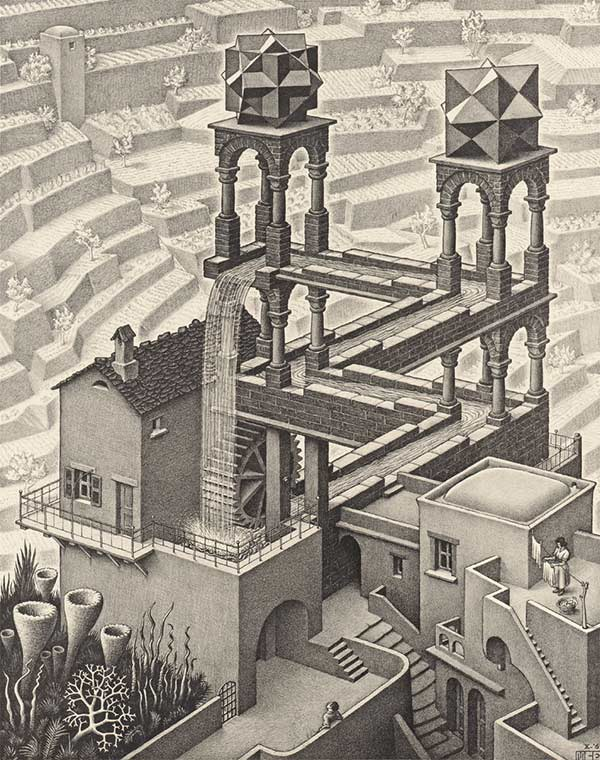
\includegraphics[scale=0.3]{img/Escher-Waterfall-1961.eps}
 \captionsetup{labelformat=empty}
 \caption{埃舍尔《瀑布》1961}
 \label{fig:Escher-Waterfall}
\end{wrapfigure}

1996年,第26界国际奥林匹克运动会正在美国的亚特兰大举行。来自世界各地的选手在速度、力量、技巧上展开竞赛挑战人类的极限。与此同时,还进行着另一场有趣的竞赛。超级计算机“深蓝”与人类的国际象棋世界冠军卡斯帕罗夫展开了对抗赛。比赛结果是深蓝2胜4负输给了人类象棋冠军。翌年,改进的深蓝再次向卡斯帕罗夫发起挑战。5月11日,计算机在正常时限的比赛中首次击败了卡斯帕罗夫。总比分1胜2负3平。深蓝计算机重1270公斤,有32个微处理器,每秒钟可以计算2亿步。为了能让"深蓝”挑战人类冠军,设计小组输入了一百多年来优秀棋手的对局两百多万对局。人类用智慧创造的机器,在人类骄傲的智慧领域首次击败了人类——这一结局引发了关注、恐惧、和激烈的讨论。

在当时,人们普遍认为,这是人工智能的一大进步。尽管在国际象棋上取得了巨大进步,但是在围棋上,计算机和人类仍存在巨大差距。对于国际象棋来说,棋盘8行8列,32枚棋子。计算机要在$10^{123}$这样巨大的博弈树中进行搜索。即使深蓝美妙能算2亿步,遍历博弈树仍需要近$10^{107}$年。为此深蓝的设计小组通过计算机程序缩小了搜索空间,使得深蓝能够搜索当前棋局后面的12步棋。而一般好的人类棋手,大约只能估计到10步左右。但是围棋的棋盘有19行19列,共361个格点上可以放黑色或者白色的棋子。博弈树的规模为$10^{360}$,远远超越国际象棋。所以在之后的一段时间里,人们仍然不相信计算机可以挑战我们。

%\begin{wrapfigure}{R}{0.5\textwidth}
\begin{figure}[htbp]
 \centering
 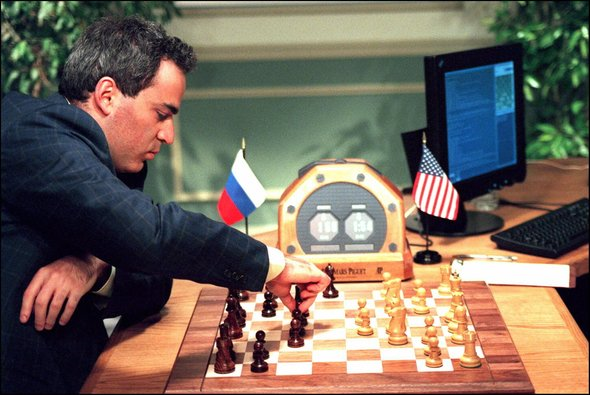
\includegraphics[scale=0.4]{img/Deep-blue-1997.eps}
 \captionsetup{labelformat=empty}
 \caption{卡斯帕罗夫在与深蓝对弈,图片原载《科学美国人杂志》}
 \label{fig:Deep-blue-1997}
\end{figure}
%\end{wrapfigure}

时光匆匆过去了20年,2016年,计算机程序Alpha-Go向人类的围棋大师展开了挑战。韩国的九段棋手李世石以1比4输掉了比赛。一年后,再次以3局全胜战胜了中国棋手柯洁。被人们认为是人工智能游戏“圣杯”的围棋终于被攻破了。作为人类,我们的心情很复杂。即使是从事智力工作的程序员群体也感到了来自机器的压力——我们是否会被机器取代?

%University of Tubingen, Germany
% Leon A. Gatys, Alexander S. Ecker Matthias Bethge
传统上我们认为,艺术文学等领域,涉及人们的文化背景、感情和性格因素,是无法被机器替代的。2015年,德国斯图加特以南40公里的小镇图宾根大学大学的盖提斯,埃克,贝特格利用机器学习人类艺术家的风格,把图宾根镇的风景照片变换成了不同风格的艺术画作。

%\begin{wrapfigure}{R}{0.5\textwidth}
\begin{figure}[htbp]
 \centering
 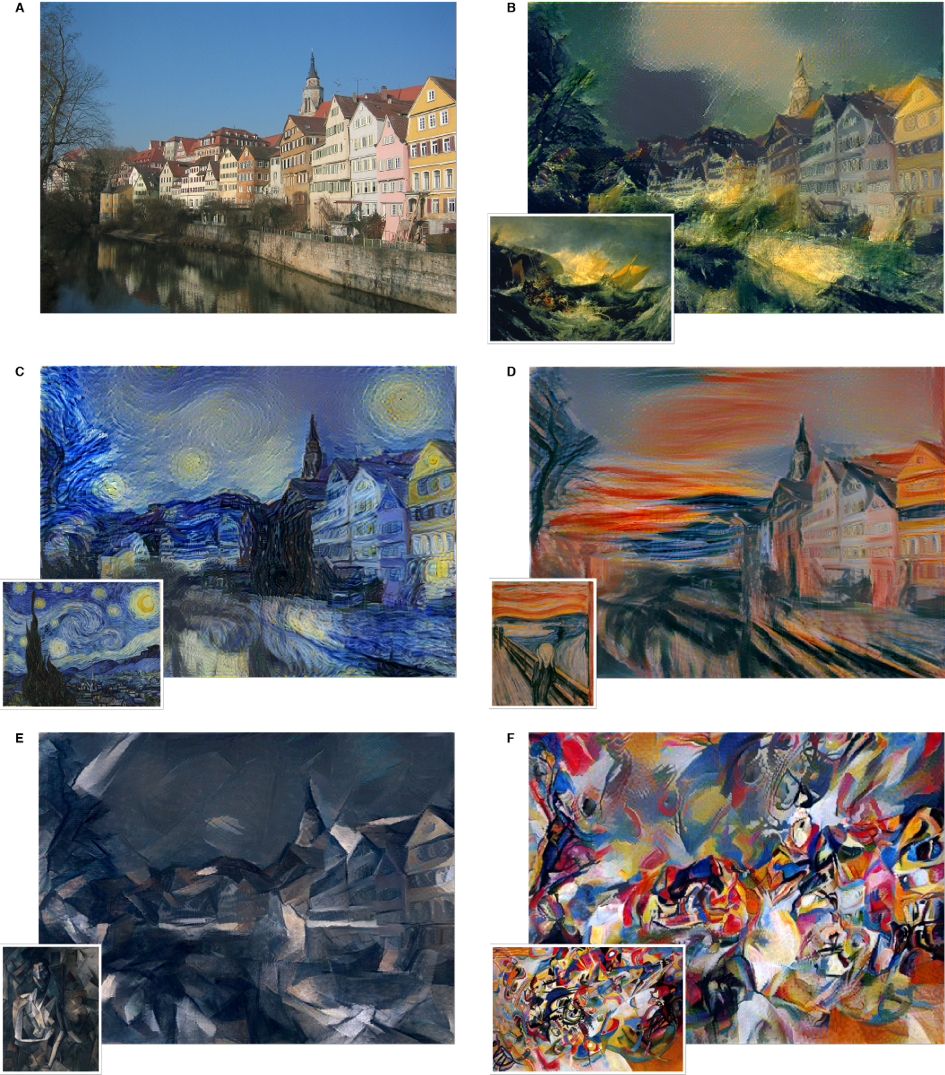
\includegraphics[scale=0.85]{img/style-transfer.eps}
 \captionsetup{labelformat=empty}
 \caption{机器学习产生的不同艺术风格的画作:A,图宾根镇的风景照片;B,英国画家透纳1810年的原作《运输船遇难》和透纳风格的画作;C,荷兰后印象派画家梵高1889年的原作《星空》和梵高风格的画作;D,挪威表现主义画家爱德华$\cdot$蒙克1893年的原作《呐喊》和蒙克风格的画作;E,西班牙现代艺术家毕加索1910年的原作《坐着的裸女》和毕加索风格的画作;F,俄罗斯抽象艺术先驱画家康定斯基1913年的原作《构成第七号》和康定斯基风格的画作}
 \label{fig:Deep-blue-1997}
\end{figure}
%\end{wrapfigure}


回顾人类面临人工智能挑战的情况,国际象棋、围棋、绘画、医疗影像判断等。
提出计算机能否战胜人类的问题

\section{计算的边界}

图灵停机问题

停机问题类比,并引出罗素悖论

\section{罗素悖论}

\section{数学基础的分歧}

逻辑主义

直觉主义

形式主义

\section{公理集合论}

\section{哥德尔不完全性定理}

\section{不完全性定理的证明}

\section{万能的程序与对角线证明}

\section{尾声}
理性思维的边界。

埃舍尔的龙

\ifx\wholebook\relax \else
\begin{thebibliography}{99}

\bibitem{De-linfini-2018}
[法] 让-皮埃尔$\cdot$卢米涅,马克$\cdot$拉雪茨-雷 著,孙展 译. 从无穷开始——科学的困惑与疆界. 人民邮电出版社. 2018. ISBN: 9787115479198

\bibitem{Noguchi2007}
[日] 野口哲也 著,刘慧 韩丽红 译. 数学原来可以这样学. 湖南人民出版社. 2014. ISBN: 9787556100897
% Tetsunori Noguchi. SUGAKUTEKI SENSE GA MINITUKU RENSHUCHO.

\bibitem{Wikipedia-Googol}
Wikipedia. ``Googol''. \url{https://en.wikipedia.org/wiki/Googol}

\bibitem{Wikipedia-Zeno}
Wikipedia. ``Zeno's Paradoxes''. \url{https://en.wikipedia.org/wiki/Zeno's_paradoxes}

\bibitem{HanXueTao16}
韩雪涛 ``数学悖论与三次数学危机''. 人民邮电出版社. 2016, ISBN: 9787115430434

\bibitem{Elements}
[古希腊] 欧几里得 著,兰纪正 朱恩宽 译,梁宗巨 张毓新 徐伯谦 校订 ``几何原本''. 译林出版社. 2014, ISBN: 9787544750066

\bibitem{M-Kline-2007}
[美] M$\cdot$克莱因 著 李宏魁 译 ``数学:确定性的丧失'' 湖南科学技术出版社,2007年4月 ISBN: 978-7-5357-1857-0
% Morris Kline ``Mathematics: The Loss of Certainty''. Oxford University Press, 1980.

\bibitem{Stepanov}
Stepanov and Rose. ``数学与泛型编程''. 爱飞翔译,机械工业出版社。ISBN: 978-7-111-57658-7. 2017.

\bibitem{GEB}
[美]候世达 ``哥德尔、埃舍尔、巴赫——集异壁之大成''. 商务印书馆 1996. ISBN: 978-7-100-01323-9

\bibitem{GCH}
张锦文,王雪生 ``连续统假设''. 世界数学名题欣赏丛书。辽宁教育出版社 1988. ISBN: 7-5382-0436-9/G$\cdot$445

\end{thebibliography}

\expandafter\enddocument
%\end{document}

\fi
